\documentclass[aspectratio=169]{beamer}

\usetheme{Boadilla}
\setbeamertemplate{navigation symbols}{}

\usepackage[T1]{fontenc}
\usepackage[utf8]{inputenc}
\usepackage{booktabs}
\usepackage{array}
\usepackage{amsmath}
\usepackage{xcolor}
\usepackage{tikz}
\usetikzlibrary{arrows.meta, positioning, fit, backgrounds, decorations.pathreplacing}

\definecolor{qNavy}{RGB}{15, 40, 90}
\definecolor{qMid}{RGB}{0, 100, 180}
\definecolor{qLight}{RGB}{220, 232, 245}
\definecolor{qGold}{RGB}{200, 160, 40}
\definecolor{qRed}{RGB}{180, 30, 30}
\definecolor{qGreen}{RGB}{20, 130, 60}

\setbeamercolor{frametitle}{bg=qNavy, fg=white}
\setbeamercolor{frametitle right}{bg=qNavy}
\setbeamercolor{title}{fg=qNavy}
\setbeamercolor{structure}{fg=qNavy}
\setbeamerfont{frametitle}{size=\normalsize, series=\bfseries}

\title[Strategy-Space Prediction]{Predicting Asset Returns via a\\Structured Strategy Space}
\subtitle{A Two-Layer Mathematical Framework for Adaptive Trading}
\author{Joon Jeremy Chun}
\date{April 27, 2026}

\begin{document}

% ── Slide 1: Title ────────────────────────────────────────────────────────────
\begin{frame}
  \titlepage
\end{frame}

% ── Slide 2: The Question ─────────────────────────────────────────────────────
\begin{frame}{The Question}

  \begin{block}{Central Question}
    Can we build a mathematically structured prediction system that
    \textbf{identifies which combination of trading signals best predicts
    near-future returns} --- and adapts as market conditions change?
  \end{block}

  \vspace{0.6em}
  \textbf{Why this is well-defined:}
  \begin{itemize}
    \item Asset: GLD (SPDR Gold ETF) --- liquid, well-studied, daily price data
    \item Prediction target: 130-day forward return (a specific, measurable quantity)
    \item ``Best'' = lowest cross-validated prediction error on held-out data
    \item ``Adapts'' = model re-estimated every month on a rolling 1-year window
  \end{itemize}

  \vspace{0.5em}
  \textbf{What makes it a math problem:}
  Two objectives — (1) optimize strategy parameters, (2) learn a sparse linear
  predictor — are composed into a single rolling estimation pipeline.

\end{frame}

% ── Slide 3: The Challenge ────────────────────────────────────────────────────
\begin{frame}{The Challenge: ML on Financial Time Series}

  \begin{columns}[T]
    \begin{column}{0.48\textwidth}
      \textbf{Problem 1: Too many features}
      \begin{itemize}
        \item Standard ML needs $n \gg d$ (data $\gg$ features)
        \item A grid search over strategy parameters produces \textbf{hundreds of candidate signals}
        \item Fitting all of them on one year of data $\Rightarrow$ severe overfitting
      \end{itemize}
    \end{column}
    \begin{column}{0.48\textwidth}
      \textbf{Problem 2: Can't just use more data}
      \begin{itemize}
        \item Financial data is \textbf{non-stationary}: regimes shift
        \item A longer training window captures outdated market behavior
        \item \emph{More data $\neq$ better model} when the process changes over time
      \end{itemize}
    \end{column}
  \end{columns}

  \vspace{0.8em}
  \begin{center}
  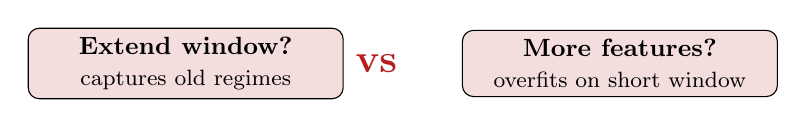
\begin{tikzpicture}
    \node[draw, rounded corners, fill=qRed!15, minimum width=4cm, minimum height=0.8cm,
          font=\small\bfseries, align=center] (p1) {Extend window?\\{\footnotesize\normalfont captures old regimes}};
    \node[right=1.5cm of p1, draw, rounded corners, fill=qRed!15, minimum width=4cm, minimum height=0.8cm,
          font=\small\bfseries, align=center] (p2) {More features?\\{\footnotesize\normalfont overfits on short window}};
    \node[right=0.7cm of p1, left=0.7cm of p2, font=\Large\bfseries, color=qRed] (vs) {vs};
  \end{tikzpicture}
  \end{center}

  \vspace{0.4em}
  \begin{center}
    \textbf{Our solution:} use \emph{domain knowledge} to structure the features
    so the linear layer remains well-conditioned on a 1-year window.
  \end{center}

\end{frame}

% ── Slide 4: Two-Layer Architecture ──────────────────────────────────────────
\begin{frame}{Our Solution: A Two-Layer Mathematical Architecture}

  \begin{center}
  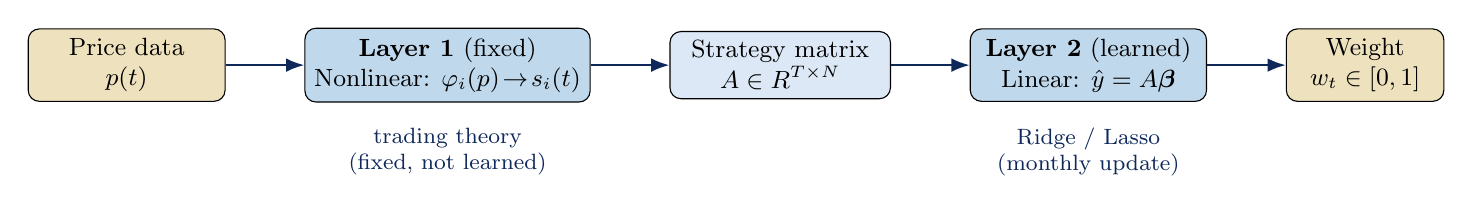
\begin{tikzpicture}[
    node distance=0.5cm and 1.0cm,
    box/.style={draw, rounded corners, minimum width=2.5cm, minimum height=0.75cm,
                align=center, font=\small},
    arrow/.style={-{Latex}, thick, color=qNavy},
  ]
    \node[box, fill=qGold!30] (price) {Price data\\$p(t)$};
    \node[box, right=of price, fill=qMid!25, minimum width=3.4cm] (layer1)
      {\textbf{Layer 1} (fixed)\\Nonlinear: $\varphi_i(p) \!\to\! s_i(t)$};
    \node[box, right=of layer1, fill=qLight, minimum width=2.8cm] (matA)
      {Strategy matrix\\$A \in \mathbb{R}^{T \times N}$};
    \node[box, right=of matA, fill=qMid!25, minimum width=3.0cm] (layer2)
      {\textbf{Layer 2} (learned)\\Linear: $\hat{y} = A\boldsymbol{\beta}$};
    \node[box, right=of layer2, fill=qGold!30, minimum width=2.0cm] (weight)
      {Weight\\$w_t \in [0,1]$};

    \draw[arrow] (price)  -- (layer1);
    \draw[arrow] (layer1) -- (matA);
    \draw[arrow] (matA)   -- (layer2);
    \draw[arrow] (layer2) -- (weight);

    \node[below=0.2cm of layer1, font=\footnotesize, color=qNavy, align=center]
      {trading theory\\(fixed, not learned)};
    \node[below=0.2cm of layer2, font=\footnotesize, color=qNavy, align=center]
      {Ridge / Lasso\\(monthly update)};
  \end{tikzpicture}
  \end{center}

  \vspace{0.5em}
  \begin{columns}[T]
    \begin{column}{0.48\textwidth}
      \textbf{Layer 1 --- Nonlinear (fixed)}
      \begin{itemize}\small
        \item Converts raw prices into \emph{structured signals}
        \item Each $\varphi_i$ is a domain-grounded function\\
              (moving averages, volatility bands, $\ldots$)
        \item Equivalent to a fixed first layer of a neural net
      \end{itemize}
    \end{column}
    \begin{column}{0.48\textwidth}
      \textbf{Layer 2 --- Linear (adaptive)}
      \begin{itemize}\small
        \item $\hat{y} = A\boldsymbol{\beta}$, learned on a rolling 1-year window
        \item Lasso drives most $\beta_i \to 0$\\
              (automatic feature selection)
        \item Re-estimated monthly $\Rightarrow$ adapts to regime shifts
      \end{itemize}
    \end{column}
  \end{columns}

\end{frame}

% ── Slide 5a: Strategy Vector Space ──────────────────────────────────────────
\begin{frame}{The Core Idea: A Strategy Vector Space}

  \begin{block}{Mathematical Foundation of Layer 1}
    Every trading strategy with parameters $\theta$ produces a signal time series
    $s_\theta(t) \in \{-1, 0, +1\}$ over $T$ days --- a \textbf{vector in $\mathbb{R}^T$}.\\[0.4em]
    The collection of all such vectors forms a \textbf{strategy vector space} $\mathcal{S}$.
  \end{block}

  \vspace{0.5em}
  \begin{columns}[T]
    \begin{column}{0.55\textwidth}
      \textbf{How we systematically span $\mathcal{S}$:}
      \begin{enumerate}\small
        \item \textbf{Grid search} over $\theta$ = sample $\mathcal{S}$ densely
        \item \textbf{Rank} by performance in selection window
        \item \textbf{Top-$N$ per family} = basis for the most\\
              performant subspace of $\mathcal{S}$
        \item \textbf{Matrix $A$} = coordinates of these basis vectors
      \end{enumerate}

      \vspace{0.5em}
      This is not arbitrary feature engineering.\\
      Each column of $A$ is a \emph{mathematically principled basis vector}
      derived from the structure of price dynamics.
    \end{column}
    \begin{column}{0.42\textwidth}
      \small
      \textbf{4 strategy families span $\mathcal{S}$:}
      \begin{itemize}
        \item Adaptive Band
        \item MA Crossover
        \item Adaptive Vol.\ Band
        \item Fear-Greed C\&V
      \end{itemize}
      \vspace{0.3em}
      $N=10$ per family $\Rightarrow$\\
      $\mathbf{A} \in \mathbb{R}^{T \times 40}$\\[0.3em]
      Monthly re-selection = subspace adapts to current regime
    \end{column}
  \end{columns}

\end{frame}

% ── Slide 5b: Strategy Examples ───────────────────────────────────────────────
\begin{frame}{Two Example Strategies from the Space}

  \begin{columns}[T]
    \begin{column}{0.48\textwidth}
      \textbf{Adaptive Band Strategy}\\
      {\footnotesize Signal: $+1$ when price crosses above upper band, $-1$ below lower band}
      \vspace{0.2em}
      \begin{center}
        \includegraphics[width=\textwidth, height=3.8cm, keepaspectratio]
          {../../figures/adaptive_band_strategy/1y/1y_rank01_ma10_uk-1.7_lk-2.0.png}
      \end{center}
    \end{column}
    \begin{column}{0.48\textwidth}
      \textbf{MA Crossover Strategy}\\
      {\footnotesize Signal: $+1$ when short MA crosses above long MA, $-1$ when crosses below}
      \vspace{0.2em}
      \begin{center}
        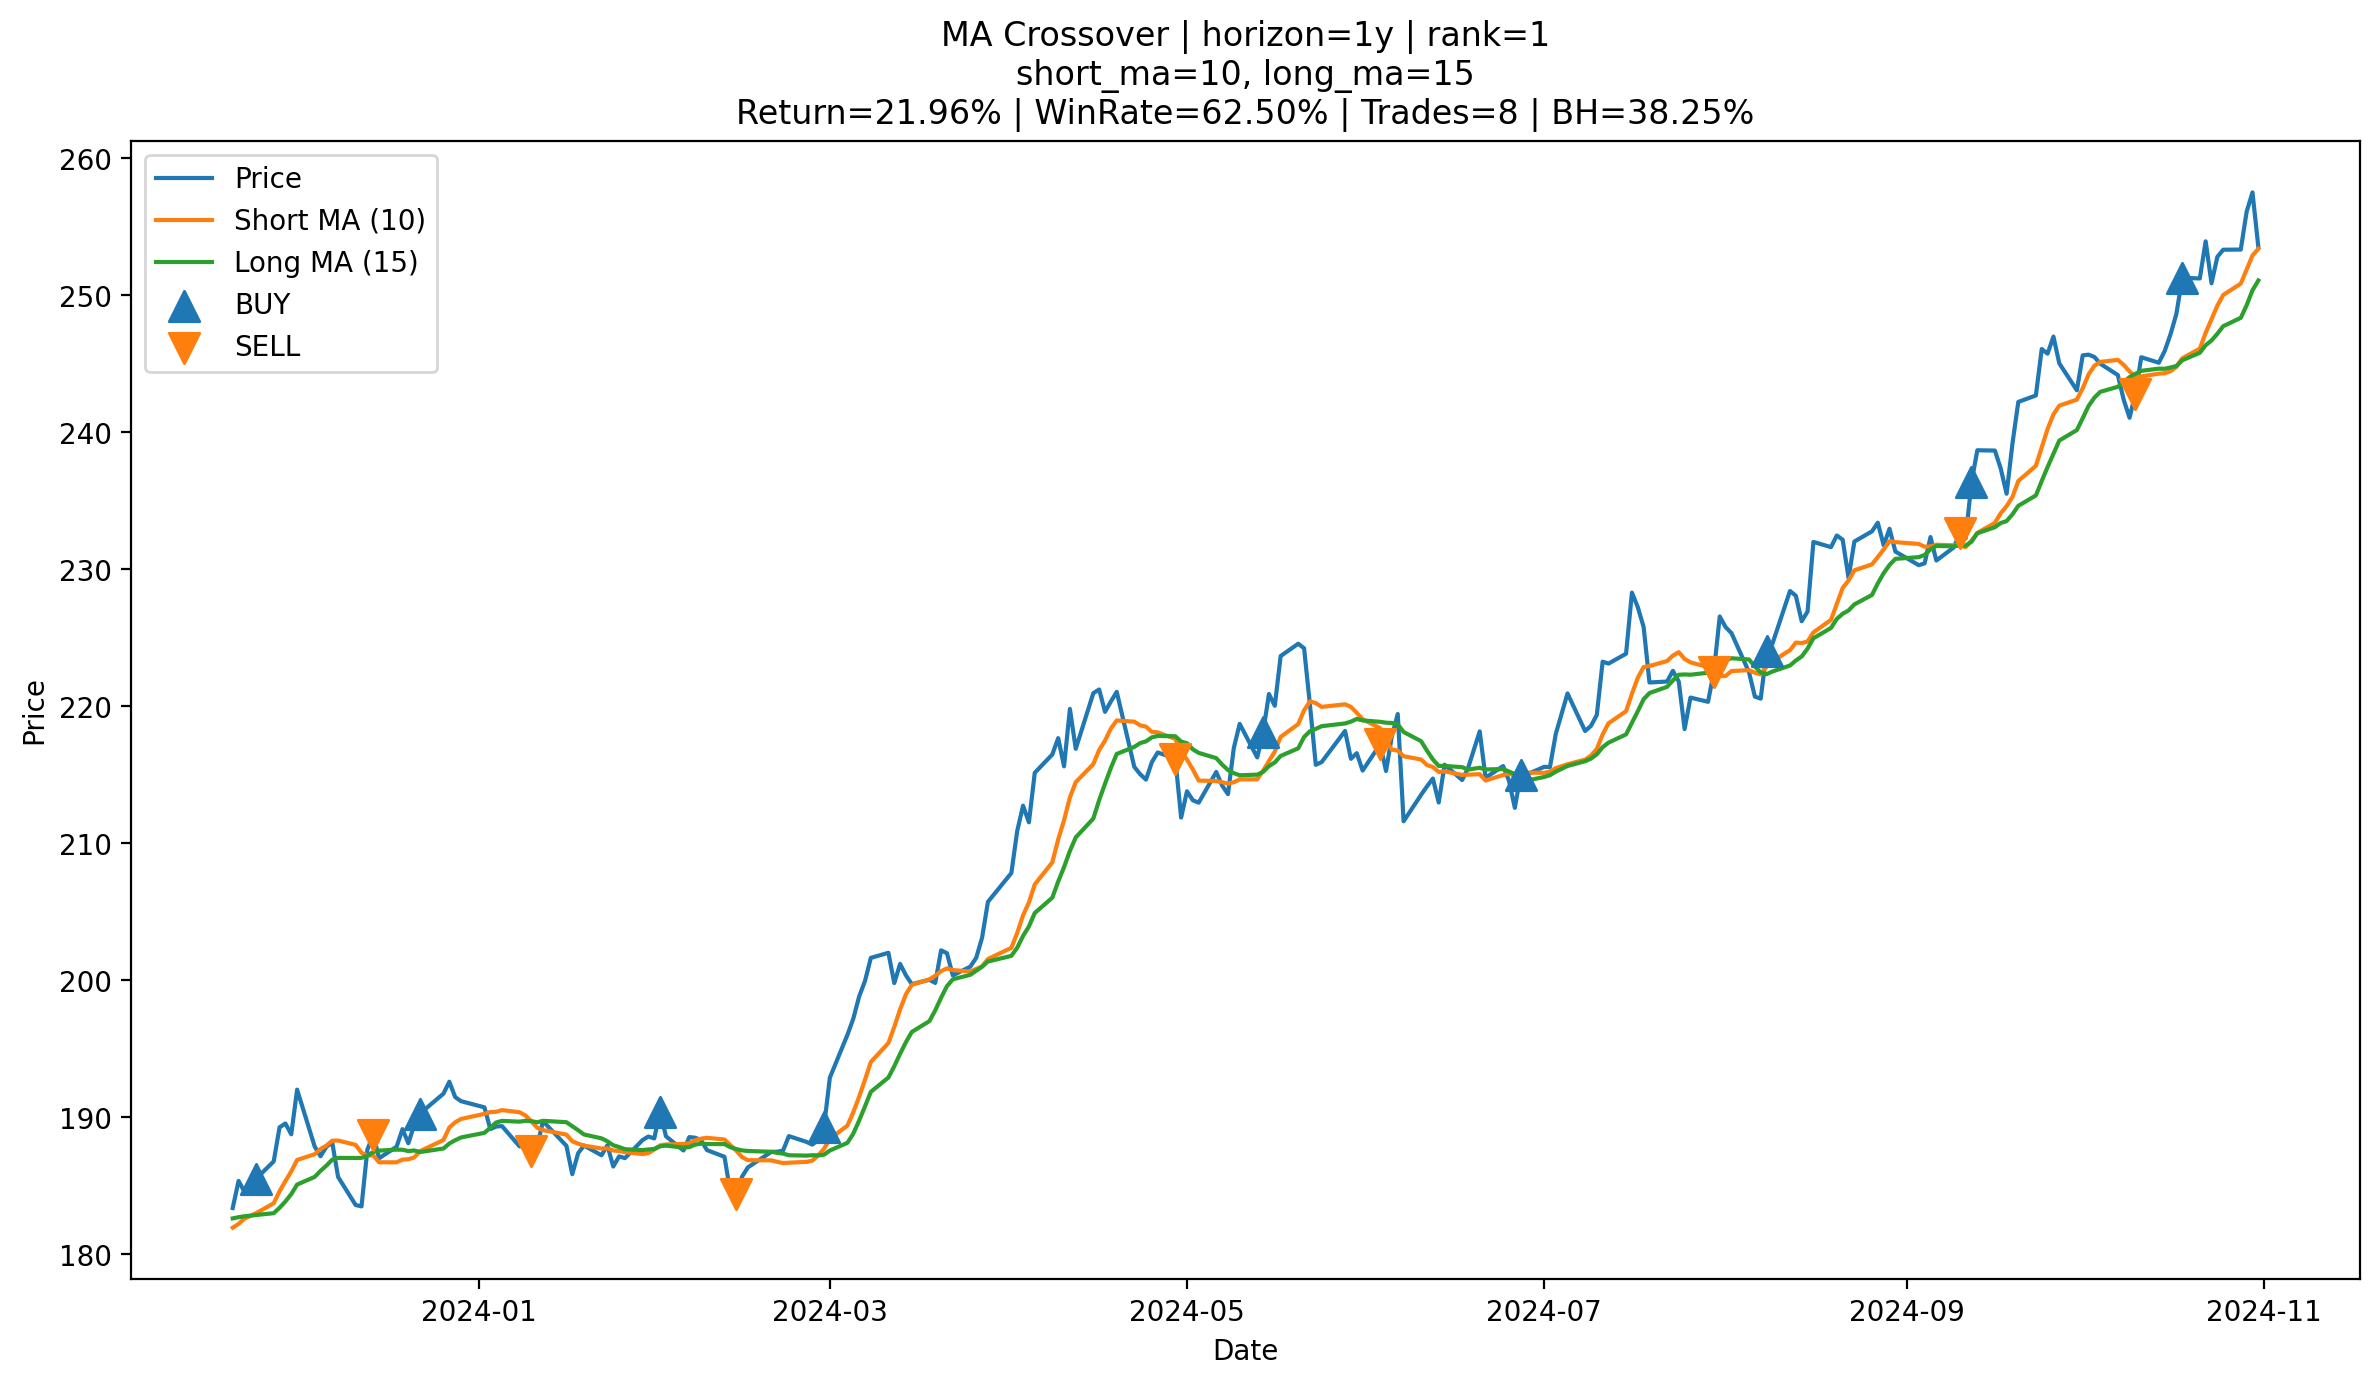
\includegraphics[width=\textwidth, height=3.8cm, keepaspectratio]
          {../../figures/ma_crossover/1y/1y_rank01_sma10_lma15.png}
      \end{center}
    \end{column}
  \end{columns}

  \vspace{0.3em}
  {\small
  Each plot shows: price (top), signal value $s_\theta(t) \in [-1, +1]$ (bottom).
  Different parameter choices $\theta$ produce different vectors in $\mathcal{S}$.
  Two more families (Adaptive Vol.\ Band, Fear-Greed) complete the basis.
  }

\end{frame}

% ── Slide 6: Three Stages of Complexity ──────────────────────────────────────
\begin{frame}{Building Complexity in Three Stages}

\small
\begin{tabular}{p{1.4cm}p{3.6cm}p{3.6cm}p{3.6cm}}
  \toprule
  & \textbf{Stage A} & \textbf{Stage B} & \textbf{Stage C} \\
  \midrule
  \textbf{Question}
    & Which single strategy works best now?
    & What weighted mix maximizes past return?
    & Which mix best \emph{predicts future} return? \\[0.3em]
  \textbf{Method}
    & Grid search,\\pick rank-1
    & Constrained opt.\\over $A\mathbf{x}$
    & Ridge / Lasso /\\ElasticNet on $A$ \\[0.3em]
  \textbf{Limit}
    & Partial signal
    & Fixed weights,\\no prediction
    & --- \\
  \bottomrule
\end{tabular}

\normalsize
\vspace{0.5em}
All three stages use the \textbf{same matrix $A$} from the strategy vector space.\\[0.3em]
Stage C asks a fundamentally different question: instead of fitting to past returns,
it fits a model to \emph{predict} the next 130-day return.

\end{frame}

% ── Slide 7: Validation Design ───────────────────────────────────────────────
\begin{frame}{Validation: Rolling Forward Test (No Look-Ahead)}

  \begin{center}
  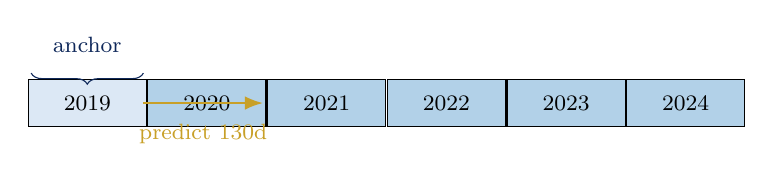
\begin{tikzpicture}[scale=0.95]
    \foreach \y/\col in {2019/qLight, 2020/qMid!30, 2021/qMid!30, 2022/qMid!30, 2023/qMid!30, 2024/qMid!30}{
      \node[draw, fill=\col, minimum width=1.5cm, minimum height=0.6cm,
            font=\footnotesize, align=center] at ({(\y-2019)*1.6}, 0) {\y};
    }
    \draw[decorate, decoration={brace, amplitude=4pt}, color=qNavy]
      (0.75, 0.4) -- (-0.75, 0.4) node[midway, above=4pt, font=\footnotesize] {anchor};
    \draw[-{Latex}, color=qGold, thick] (0.75, 0) -- (2.35, 0)
      node[midway, below=4pt, font=\footnotesize, color=qGold] {predict 130d};
  \end{tikzpicture}
  \end{center}

  \vspace{0.3em}
  \begin{enumerate}
    \item \textbf{Anchor date} (e.g., 2020-12-31): grid-search strategy parameters on the past year
    \item \textbf{Model selection}: fit Ridge/Lasso/ElasticNet on anchor window; pick by CV-MSE
    \item \textbf{Hold}: deploy signal for 130 days, then recycle capital into the next tranche
    \item \textbf{Update}: at next month's anchor, re-run steps 1--3
  \end{enumerate}

  \vspace{0.4em}
  \textbf{79 anchor dates} (2019-12 to 2026-03) covering the full evaluation period.\\
  \textbf{Forward test: 2020--2024} --- all decisions made with data available at the time.

  \vspace{0.3em}
  \begin{block}{}
    \small
    The tranche structure ensures capital is continuously deployed:
    each day one of the 130 open tranches matures and is reinvested.
  \end{block}

\end{frame}

% ── Slide 8: Three-Stage Results ─────────────────────────────────────────────
\begin{frame}{Results: Stages A, B, and C Compared}

  \small
  Hold 130d $\cdot$ 1M update $\cdot$ GLD 2020--2024 \quad {\footnotesize(Ret / Avg.Exp)}

  \vspace{0.3em}
  \begin{tabular}{lrrrr}
    \toprule
    Year & B\&H & \textbf{A}: Single & \textbf{B}: Ensemble & \textbf{C}: ML-Guided \\
    \midrule
    2020 & $+$23.9\% & $+$4.4\% / 27\% exp & $+$6.4\% / 32\% exp & \textbf{$+$10.9\%} / 57\% exp \\
    2021 & $-$6.2\%  & $+$0.3\% / 25\%     & $+$0.3\% / 25\%     & \textbf{$+$0.8\%}  / 29\% \\
    2022 & $+$0.8\%  & $-$0.9\% / 46\%     & $-$2.3\% / 42\%     & \textbf{$-$0.2\%}  / 31\% \\
    2023 & $+$11.8\% & $+$1.6\% / 25\%     & $+$2.0\% / 23\%     & \textbf{$+$4.0\%}  / 32\% \\
    2024 & $+$27.0\% & $+$5.9\% / 21\%     & $+$8.0\% / 29\%     & \textbf{$+$16.4\%} / 65\% \\
    \midrule
    \textbf{Sharpe (eff.)} & --- & $\approx$0.5 & $\approx$0.7 & \textbf{1.08} \\
    \bottomrule
  \end{tabular}

  \vspace{0.4em}
  \begin{itemize}
    \item Stage C \textbf{best in every year} on both return and capital efficiency
    \item 2024: A($+$5.9\%) $\to$ B($+$8.0\%) $\to$ C($+$16.4\%) --- clear step-up at each stage
    \item ML-Guided model learns \emph{when} and \emph{how much} to invest, not just which strategy
    \item 2021 bear year: Stage C still positive ($+$0.8\%) while B\&H lost $-$6.2\%
  \end{itemize}

\end{frame}

% ── Slide 9: Key Insight — Why 130 Days ──────────────────────────────────────
\begin{frame}{Key Insight: Why Does 130 Days Work Best?}

  \textbf{Horizon scan} --- we tested every prediction target from 5 to 260 days.
  \textbf{130 days (6 months)} was most consistently selected.

  \vspace{0.4em}
  \begin{block}{The alignment insight}
    Stage A/B optimize strategy parameters using a \textbf{6-month evaluation window}
    ($\approx$130 trading days).
    When Layer 2 predicts \emph{the same 130-day horizon}, the features in matrix $A$
    are calibrated to exactly the scale the model is trying to predict.
    \textbf{Feature--target alignment}.
  \end{block}

  \vspace{0.4em}
  \textbf{Evidence --- dedicated model comparison (2020--2024):}

  \vspace{0.2em}
  \begin{tabular}{lrrrrrr}
    \toprule
    Model & 2020 & 2021 & 2022 & 2023 & 2024 & Sharpe \\
    \midrule
    \textbf{h130} (train 130d, hold 130d)
      & $+$19\% & \textbf{$+$3\%} & $-$1\% & $+$13\% & $+$25\% & \textbf{1.08} \\
    h45  (train 45d, hold 45d)
      & $+$19\% & \textcolor{qRed}{\textbf{$-$18\%}} & $-$5\% & $+$6\% & $+$29\% & \textcolor{qRed}{0.33} \\
    \bottomrule
  \end{tabular}

  \vspace{0.3em}
  {\footnotesize Values are capital efficiency = return $\div$ average exposure.}

  \vspace{0.3em}
  \begin{itemize}
    \item h45 catastrophically fails in a bear year (2021: $-$18\% efficiency)
    \item Shorter-horizon targets are noisier $\Rightarrow$ poor generalization in adversarial markets
  \end{itemize}

\end{frame}

% ── Slide 10: Live System ─────────────────────────────────────────────────────
\begin{frame}{Stage C in Production: Live Signal}

  \textbf{Deployed on Raspberry Pi} --- runs every trading day at 13:00 PDT

  \vspace{0.4em}
  \begin{center}
  \begin{tabular}{ll}
    \toprule
    \multicolumn{2}{c}{\textbf{GLD Signal --- as of 2026-04-24}} \\
    \midrule
    Signal              & \textbf{BUY (strong)} \\
    Target Weight       & 1.00 \quad (full position) \\
    Predicted Return    & $+$55.6\% over 130 days \\
    Active Model        & Ridge \\
    Active Anchor       & 2026-03-31 \\
    Dominant Family     & MA Crossover \\
    \bottomrule
  \end{tabular}
  \end{center}

  \vspace{0.5em}
  \begin{columns}[T]
    \begin{column}{0.5\textwidth}
      \textbf{Pipeline (automated):}
      \begin{enumerate}\small
        \item Fetch latest GLD price (Alpaca API)
        \item Re-run Layer 1 with current anchor
        \item Layer 2 predicts $\hat{y}$ $\to$ weight $w_t$
        \item Execute tranche order (paper trading)
        \item Push signal to GitHub
      \end{enumerate}
    \end{column}
    \begin{column}{0.5\textwidth}
      \textbf{Infrastructure:}
      \begin{itemize}\small
        \item Raspberry Pi 4 (always-on, low power)
        \item Alpaca paper trading account
        \item Systemd timer: runs Mon--Fri only
        \item Email alert with full report sent daily
        \item Signal JSON committed to git automatically
      \end{itemize}
    \end{column}
  \end{columns}

\end{frame}

% ── Slide 11: Conclusion ──────────────────────────────────────────────────────
\begin{frame}{Conclusion: Back to the Question}

  \begin{block}{We asked:}
    Can a structured mathematical framework identify which trading signal
    combinations best predict near-future returns --- and adapt as markets change?
  \end{block}

  \vspace{0.5em}
  \begin{block}{We found: \textbf{Yes.}}
    \begin{itemize}
      \item \textbf{Two-layer structure} solves the ML challenge: domain-knowledge features
            (Layer 1) keep the linear layer well-conditioned on a 1-year window
      \item \textbf{Monthly rolling re-estimation} captures regime shifts without
            sacrificing statistical stability
      \item \textbf{130-day horizon} is the sweet spot: feature--target alignment
            between Layer 1 optimization and Layer 2 prediction
      \item \textbf{Stage C dominates A and B} in every year of the 5-year forward test
            (Sharpe 1.08 vs.\ $\approx$0.5--0.7)
      \item The system is \textbf{live and running} on real market data today
    \end{itemize}
  \end{block}

  \vspace{0.3em}
  \textbf{What's next:} extend to multiple assets simultaneously ---
  if GLD and Berkshire Hathaway signals are uncorrelated,
  idle capital from one asset can be deployed into the other.

\end{frame}

% ── Backup / Q&A ─────────────────────────────────────────────────────────────
\begin{frame}{}
  \begin{center}
    \vspace{1cm}
    {\Large \textbf{Thank you}}\\[1em]
    {\normalsize Questions welcome}\\[2em]
    {\small Appendix slides follow for detailed results}
  \end{center}
\end{frame}

% =============================================================================
% APPENDIX
% =============================================================================
\appendix

\begin{frame}{Appendix A: Detailed Results — Stage C h130 (top-10)}
  \small
  Return / Avg.\ Exposure / Capital Efficiency = Return $\div$ Exposure

  \vspace{0.4em}
  \begin{tabular}{lrrrrr}
    \toprule
    Year & B\&H & Strategy Ret & Avg.\ Exp & Efficiency & vs.\ B\&H \\
    \midrule
    2020 & $+$23.9\% & $+$10.9\% & 57\% & $+$19\% & $-$13.0\%p \\
    2021 & $-$6.2\%  & $+$0.8\%  & 29\% & $+$3\%  & $+$7.0\%p  \\
    2022 & $+$0.8\%  & $-$0.2\%  & 31\% & $-$1\%  & $-$1.0\%p  \\
    2023 & $+$11.8\% & $+$4.0\%  & 32\% & $+$13\% & $-$7.8\%p  \\
    2024 & $+$27.0\% & $+$16.4\% & 65\% & $+$25\% & $-$10.6\%p \\
    \midrule
    5yr total & $+$66.3\%  & $+$36.4\%  & avg 43\% & $+$11.7\%  & \\
    Sharpe    & ---        & ---        &          & 1.08       & \\
    \bottomrule
  \end{tabular}

  \vspace{0.4em}
  \textbf{Interpretation}: Strategy return is lower than B\&H but uses only 43\% of capital on average.
  Idle capital (57\%) can be deployed elsewhere --- efficiency per deployed dollar exceeds B\&H.
\end{frame}

\begin{frame}{Appendix B: h130 vs h45 Full Comparison (top-10)}
  \small
  Capital Efficiency = Return $\div$ Avg.\ Exposure

  \vspace{0.3em}
  \begin{tabular}{lrrrrrr}
    \toprule
    & 2020 & 2021 & 2022 & 2023 & 2024 & Sharpe \\
    \midrule
    \textbf{h130} eff & $+$19\% & $+$3\% & $-$1\% & $+$13\% & $+$25\% & \textbf{1.08} \\
    h45 eff  & $+$19\% & \textcolor{qRed}{$-$18\%} & $-$5\% & $+$6\% & $+$29\% & \textcolor{qRed}{0.33} \\
    \midrule
    \textbf{h130} ret & $+$10.9\% & $+$0.8\% & $-$0.2\% & $+$4.0\% & $+$16.4\% & \\
    h45 ret  & $+$11.1\% & \textcolor{qRed}{$-$9.9\%} & $-$1.6\% & $+$4.3\% & $+$24.1\% & \\
    \midrule
    B\&H & $+$23.9\% & $-$6.2\% & $+$0.8\% & $+$11.8\% & $+$27.0\% & \\
    \bottomrule
  \end{tabular}

  \vspace{0.4em}
  h45 outperforms in bull years (2024: $+$29\% vs $+$25\% eff) but
  catastrophically fails in bear year (2021: $-$18\% vs $+$3\%).
  The feature--target misalignment amplifies noise in adversarial conditions.
\end{frame}

\begin{frame}{Appendix C: Update Frequency (Stage C, h130)}
  \small
  Return / Avg.\ Exposure --- more frequent updates generally improve performance

  \vspace{0.3em}
  \begin{tabular}{lrrrrr}
    \toprule
    Year & B\&H & 1M update & 2M update & 3M update & 6M update \\
    \midrule
    2020 & $+$23.9\% & $+$10.9\% / 57\% & $+$10.2\% / 57\% & $+$9.6\% / 51\% & $+$9.7\% / 50\% \\
    2021 & $-$6.2\%  & $+$0.8\% / 29\%  & $+$0.3\% / 35\%  & $+$0.6\% / 28\% & $-$0.7\% / 49\% \\
    2022 & $+$0.8\%  & $-$0.2\% / 31\%  & $+$0.9\% / 35\%  & $-$0.8\% / 33\% & $-$1.7\% / 44\% \\
    2023 & $+$11.8\% & $+$4.0\% / 32\%  & $+$4.1\% / 23\%  & $+$3.8\% / 40\% & $+$3.4\% / 15\% \\
    2024 & $+$27.0\% & $+$16.4\% / 65\% & $+$13.9\% / 60\% & $+$11.1\% / 53\% & $+$5.5\% / 36\% \\
    \bottomrule
  \end{tabular}

  \vspace{0.3em}
  Monthly (1M) update consistently best --- model stays close to current regime.
  6M update misses regime shifts: negative in 2021 and 2022.
\end{frame}

\begin{frame}{Appendix D: Strategy Parameter Ranges (Grid Search)}
  \small
  \begin{tabular}{p{3.5cm}p{3.0cm}p{6.0cm}}
    \toprule
    Strategy & Parameter & Range \\
    \midrule
    Adaptive Band
      & MA window \newline Upper $k$ \newline Lower $k$
      & 5, 10, 22, 65, 130, 260 days \newline $-3.0$ to $+3.0$ (step 0.1) \newline $-3.0$ to $+3.0$ (step 0.1) \\
    \midrule
    MA Crossover
      & Short MA \newline Long MA
      & 5 to 95 days (step 5) \newline short$+$5 to 140 days \\
    \midrule
    Adaptive Vol.\ Band
      & MA window \newline Vol multiplier
      & 5, 10, 22, 65, 130, 260 days \newline $0.5$ to $3.0$ (step 0.1) \\
    \midrule
    Fear-Greed C\&V
      & Candle threshold \newline Volume threshold
      & $0.3\sigma$ to $2.0\sigma$ \newline $1.0\times$ to $3.0\times$ avg \\
    \bottomrule
  \end{tabular}

  \vspace{0.4em}
  Grid search runs in parallel via \texttt{joblib} (4.4$\times$ speedup, 20-core CPU).
  Top-$N$ per family selected by total return in the 1-year selection window.
\end{frame}

\end{document}
